\documentclass{beamer}
\usetheme{metropolis}

\usepackage{luatexja}
\usepackage[ipaex]{luatexja-preset}
\usepackage{listings}
\renewcommand{\kanjifamilydefault}{\gtdefault}

\title{\bfseries ISUCON本ゆる輪読会 \#4}
\subtitle{\bfseries Chapter5 データベースのチューニング}
\author{aoshima}
\date{2022年9月8日}
\subject{データベースのチューニング}

\begin{document}

\begin{frame}
  \titlepage
\end{frame}

\begin{frame}{今日の資料}
  演習で使うからcloneしておいてね!
  \href{https://github.com/aoshimash/techresi-isucon-workshop}{https://github.com/aoshimash/techresi-isucon-workshop}
\end{frame}

\begin{frame}{準備}
  今日の演習は \href{https://multipass.run/}{multipass} で \href{https://github.com/catatsuy/private-isu}{private-isu}環境を作成してそこで行います。\par
  "../enshu/private-isu/README.md" の手順に沿ってmultipassでVMを作成してください。\newline
  (こっちからでも見えます。\href{https://github.com/aoshimash/techresi-isucon-workshop/blob/main/ch5/enshu/private-isu/README.md}{https://github.com/aoshimash/techresi-isucon-workshop/blob/main/ch5/enshu/private-isu/README.md})
\end{frame}

\begin{frame}{データベースの種類}

  \begin{description}
    \item[RDBMS]SQLによる問い合わせや、強い一貫性が特徴。\\(例: MySQL, MariaDB, PostgreSQL, SQLite, RDS)
    \item[NoSQL]リレーショナルデータベース以外のデータベースシステムの総称。スケールさせやすいものが多い。\\(例: memcached, Redis, MongoDB, DynamoDB)
    \item[NewSQL]RDBMSの特徴を持ったまま、スケールさせることができるらしい。使ったことないからよく知らない。\\(例: Cloud Spanner, TiDB, Cockroach DB)
  \end{description}

  今日はRDMBSの話。

\end{frame}

\begin{frame}[fragile]{OSから負荷を観察する}
  htopでOSの負荷を観測しつつベンチマーカーを走らせてみる。\par
  まずは、VMにログインしてhtopを起動しておく。
  \begin{lstlisting}[language=bash, basicstyle=\tiny]
    multipass shell private-isu
    htop
  \end{lstlisting}
  ターミナルで別のタブを開いてベンチマーカーを実行。
  \begin{lstlisting}[language=bash, basicstyle=\tiny]
    multipass shell private-isu
    cd /home/isucon/private_isu.git/benchmarker
    ./bin/benchmarker -u ./userdata -t http://localhost/
  \end{lstlisting}
  htopを起動しているタブに戻ってOSの負荷を観測してみる
\end{frame}

\begin{frame}
  mysqlの負荷が高いことがわかる
  \begin{figure}
    \centering
    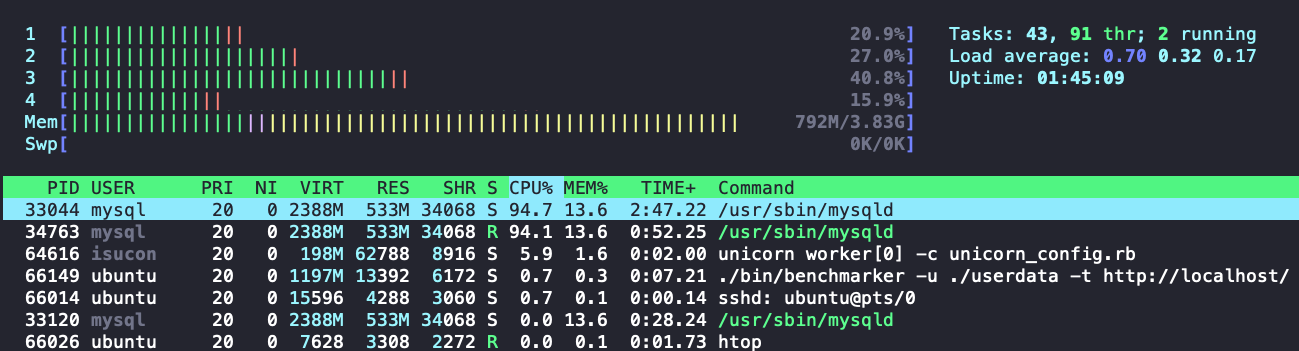
\includegraphics[clip, keepaspectratio, width=110mm]{./fig/htop.png}
  \end{figure}
\end{frame}

\begin{frame}[fragile]{MySQLのプロセスリスト}
  今度はMySQL上でどんなプロセスが動いているのか確認する。\par
  またターミナルに新たなタブを作成し、mysqlにログインする。
  \begin{lstlisting}[language=bash]
    multipass shell private-isu
    sudo mysql -u root -proot
    mysql> SHOW PROCESSLIST;
  \end{lstlisting}
  ただし、MySQLへのアクセスがない状態だとプロセスリストを見てもあんまり面白くないので、ベンチマーカーを実行しながら、プロセスリストを確認してみよう。
\end{frame}

\begin{frame}
  \begin{figure}
    \centering
    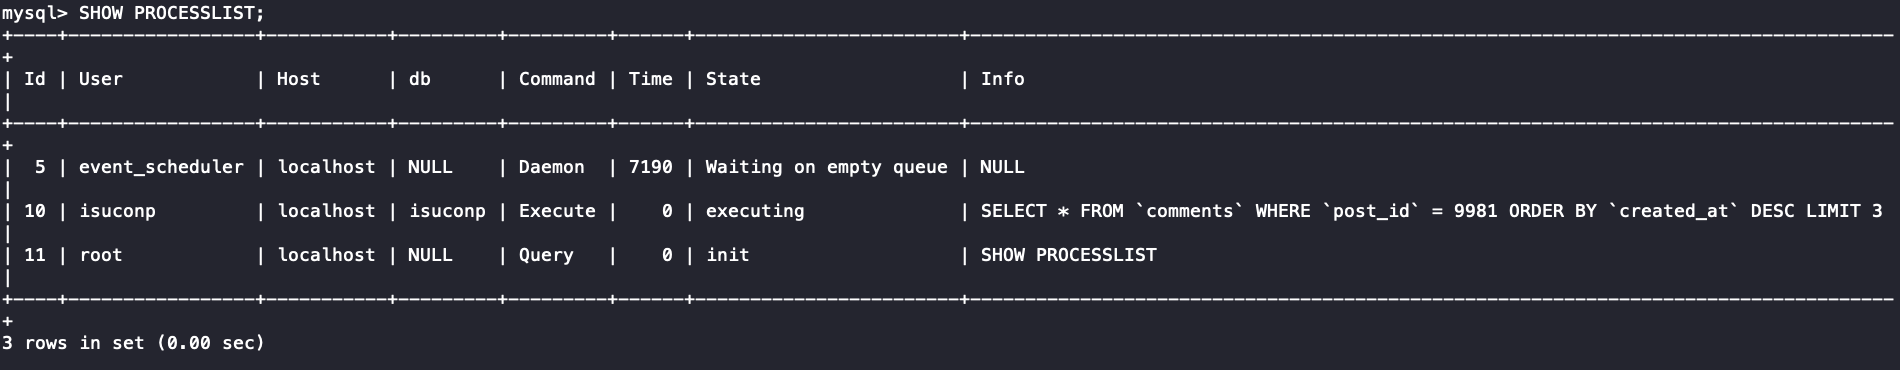
\includegraphics[clip, keepaspectratio, width=110mm]{./fig/mysql_process_list.png}
  \end{figure}
  SHOW PROCESSLIST が実行された瞬間の情報しかわからないので、大量のクエリを網羅的に解析するのには向いていない。
\end{frame}

\begin{frame}[fragile]{スロークエリログの出力設定の確認}
  まずは、現在のスロークエリログの出力設定を確認する。\par
  \begin{lstlisting}[basicstyle=\tiny]
    mysql> SHOW GLOBAL VARIABLES LIKE 'slow_query_log';
    +----------------+-------+
    | Variable_name  | Value |
    +----------------+-------+
    | slow_query_log | OFF   |
    +----------------+-------+
    1 row in set (0.00 sec)
  \end{lstlisting}
\end{frame}

\begin{frame}[fragile]{スロークエリログの出力設定}
  スロークエリログの出力設定をする。\par
  "/etc/mysql/my.cnf"をエディタで開いて、次の内容を末尾に追記する。
  \begin{lstlisting}[basicstyle=\tiny]
    [mysqld]
    # スロークエリログを有効にする
    slow_query_log = 1

    # スロークエリログの出力先
    slow_query_log_file = /var/log/mysql/mysql-slow.log

    # 指定した秒数以上かかったクエリのみログに出力する(0なので全クエリをログに出力)
    long_query_time = 0
  \end{lstlisting}

  ファイルを編集したらmysqlを再起動して設定を反映する。

  \begin{lstlisting}[basicstyle=\tiny]
    sudo systemctl restart mysql
  \end{lstlisting}

\end{frame}

\begin{frame}[fragile]{スロークエリログの出力設定の再確認}
  スロークエリログの出力設定がちゃんと反映されているか確認する。\par
  \begin{lstlisting}[basicstyle=\tiny]
    mysql> SHOW GLOBAL VARIABLES LIKE 'slow_query_log';
    +----------------+-------+
    | Variable_name  | Value |
    +----------------+-------+
    | slow_query_log | ON    |
    +----------------+-------+
    1 row in set (0.01 sec)

    mysql> SHOW GLOBAL VARIABLES LIKE 'slow_query_log_file';
    +---------------------+---------------------------------+
    | Variable_name       | Value                           |
    +---------------------+---------------------------------+
    | slow_query_log_file | /var/log/mysql/mysql−slow.log   |
    +---------------------+---------------------------------+
    1 row in set (0.01 sec)

    mysql> SHOW GLOBAL VARIABLES LIKE 'long_query_time';
    +-----------------+----------+
    | Variable_name   | Value    |
    +-----------------+----------+
    | long_query_time | 0.000000 |
    +-----------------+----------+
    1 row in set (0.00 sec)
  \end{lstlisting}
\end{frame}

\begin{frame}[fragile]{スロークエリログを取得する}
  ベンチマーカーを回す前にログファイルをローテートして、
  \begin{lstlisting}[basicstyle=\tiny]
    sudo mv /var/log/mysql/mysql−slow.log /var/log/mysql/mysql−slow.log.bak1
    sudo systemctl restart mysql
  \end{lstlisting}

  "/home/isucon/private\_isu.git/benchmarker" ディレクトリで以下を実行。

  \begin{lstlisting}[basicstyle=\tiny]
    ./bin/benchmarker -u ./userdata -t http://localhost/
  \end{lstlisting}

  そして、スロウクエリログファイルを分析した結果をファイルに出力する
  \begin{lstlisting}[basicstyle=\tiny]
    sudo pt-query-digest /var/log/mysql/mysql−slow.log > ~/pt-query-digest.log2
    less ~/pt-query-digest.log2
  \end{lstlisting}

\end{frame}

\begin{frame}{pt-query-logの結果の見方}
  pt-query-logの結果は大きく分けて3部構成になっており、上から全体的な統計、ランキング、各クエリの詳細になっている。
  まずはランキングに注目してみる。
  \begin{figure}
    \centering
    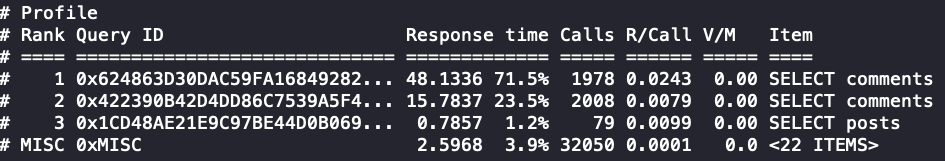
\includegraphics[clip, keepaspectratio, width=110mm]{./fig/rank_query.png}
  \end{figure}
  "Response time"が実行時間の合計と全体に占める割合。"Calls"が実行された回数。"R/Call"が1回あたりの時間。
  次はランク1位のクエリの詳細を見ていく。
\end{frame}

\begin{frame}{pt-query-logの結果の詳細}
  \begin{figure}
    \centering
    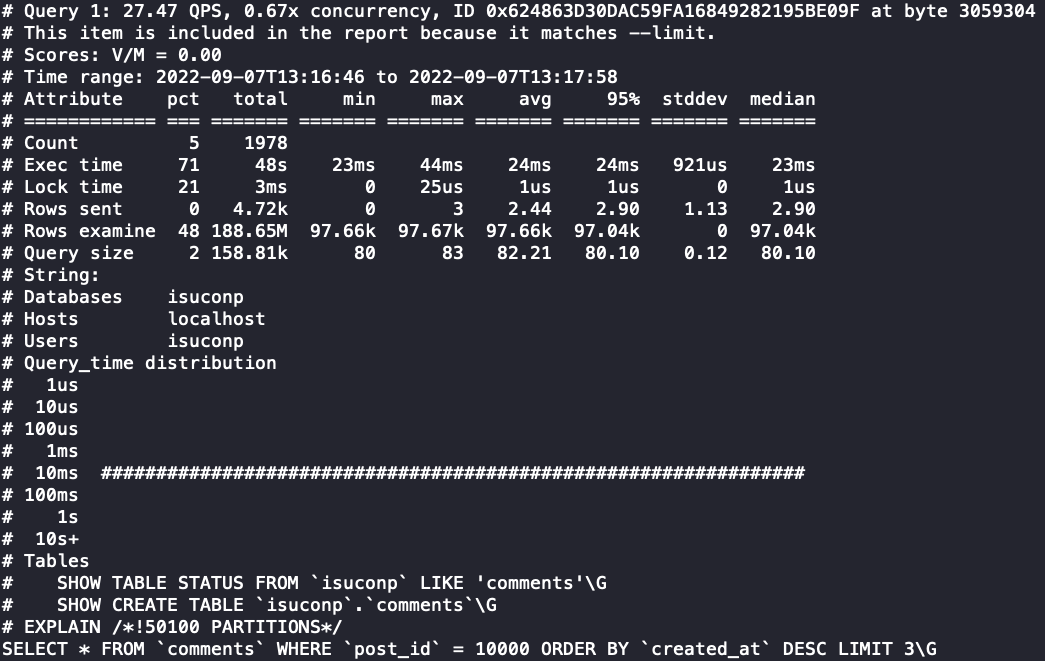
\includegraphics[clip, keepaspectratio, width=110mm]{./fig/select_query.png}
  \end{figure}
\end{frame}

\begin{frame}{pt-query-logの結果の詳細}
  \begin{description}
    \item[Count] 解析対象期間中に実行されたクエリ数
    \item[Exec time] クエリの実行にかかった時間
    \item[Lock time] クエリの実行までにかかった時間。他のスレッドによるロックの待ち時間。
    \item[Rows sent] クエリを実行し、クライアントに返した行数。
    \item[Rows examine] クエリの実行に走査した行数
    \item[Query size] 実行したクエリの長さ(文字数)
  \end{description}
\end{frame}

\begin{frame}{pt-query-logの結果の詳細}
  \begin{figure}
    \centering
    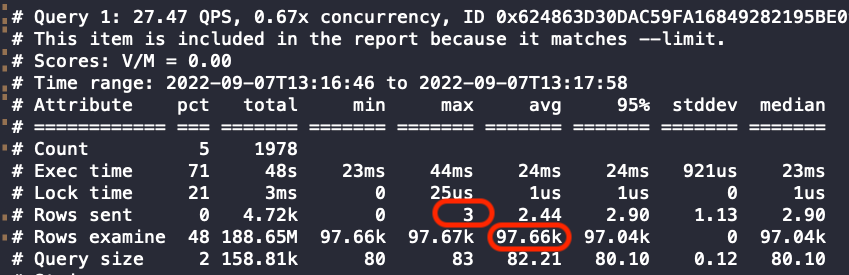
\includegraphics[clip, keepaspectratio, width=110mm]{./fig/select_query_zoom.png}
  \end{figure}
  つまり、このクエリは1978回呼び出されており、合計で48秒かかっているが、Lock timeは3msほどで小さいということがわかります。
  そして、今回注目するところは、Rows sentとRows examineの差です。
  クエリには"LIMIT 3"がついているので、1クエリで最大でも3行しか返さないのに、平均して97.66k行も処理していることがわかります。
\end{frame}

\begin{frame}[fragile]{インデックスを付与する}
  一番遅いクエリがわかったので、これを改善していく。
  \begin{lstlisting}[basicstyle=\tiny]
    SELECT * FROM `comments` WHERE `post_id` = 10000 ORDER BY `created_at` DESC LIMIT 3\G
  \end{lstlisting}
  commentsテーブルからpost\_idで検索をするのが遅いのであれば、post\_idにインデックスを貼れば解決するのではないかと推測ができる。
  \begin{lstlisting}[basicstyle=\tiny]
    mysql> use isuconp;
    mysql> ALTER TABLE `comments` ADD INDEX `post_id_idx`(`post_id`);
  \end{lstlisting}
  これで改善されたはず。
\end{frame}

\begin{frame}[fragile]{再度ベンチマーカーを回す}
  まずは、ログのローテーション
  \begin{lstlisting}[basicstyle=\tiny]
    sudo mv /var/log/mysql/mysql−slow.log /var/log/mysql/mysql−slow.log.bak2
    sudo systemctl restart mysql
  \end{lstlisting}

  "/home/isucon/private\_isu.git/benchmarker" ディレクトリで以下を実行。

  \begin{lstlisting}[basicstyle=\tiny]
    ./bin/benchmarker -u ./userdata -t http://localhost/
  \end{lstlisting}

  そして、スロウクエリログファイルを分析した結果をファイルに出力する
  \begin{lstlisting}[basicstyle=\tiny]
    sudo pt-query-digest /var/log/mysql/mysql−slow.log > ~/pt-query-digest.log3
    less ~/pt-query-digest.log3
  \end{lstlisting}

\end{frame}

\begin{frame}{結果が改善されているか確認}
  \begin{figure}
    \centering
    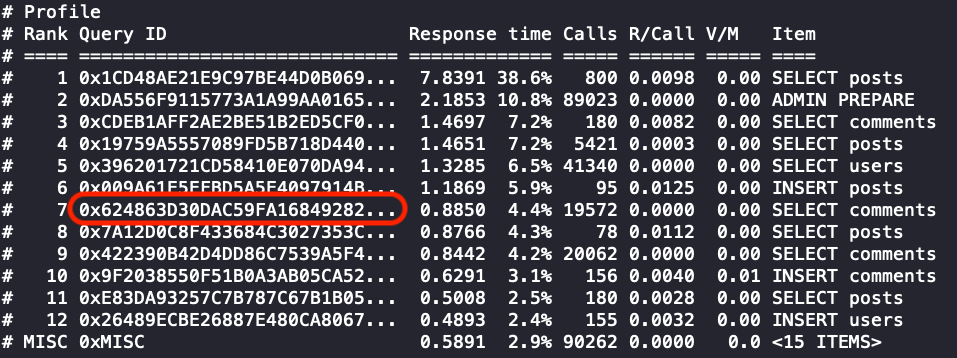
\includegraphics[clip, keepaspectratio, width=110mm]{./fig/rank_query_2.png}
  \end{figure}
  最初にランク1位だったクエリが7位まで落ちた!
\end{frame}


\end{document}
